\chapter{\IfLanguageName{dutch}{Stand van zaken}{State of the art}}
\label{ch:stand-van-zaken}

% Tip: Begin elk hoofdstuk met een paragraaf inleiding die beschrijft hoe
% dit hoofdstuk past binnen het geheel van de bachelorproef. Geef in het
% bijzonder aan wat de link is met het vorige en volgende hoofdstuk.

% Pas na deze inleidende paragraaf komt de eerste sectiehoofding.

Dit onderzoek zal zich focussen op z/OS Health Checker dit is een tool die draait in een mainframe omgeving maar vooraleer we kunnen beginnen met het bespreken van de oplossingsmethode van de onderzoeksvragen moeten we ons eerst verdiepen in de mainframe zelf en de omgeving waarin z/OS Health Checker draait om zo duidelijk te maken waarom deze tool zijn aanwezigheid belangrijk is en hoe deze werkt. Verder moeten we ook de basis begrijpen van andere tools en systemen binnen de mainframe zoals ISPF, SDS en JES. Om daarna te eindigen met JCL de taal die word gebruikt om de z/OS Health checker logs op te stellen.

\section{De Mainframe}
\label{sec:De Mainframe}

De Mainframe speelt een centrale rol in de dagelijkse operaties bij de meeste grote bedrijven. De Ontwikkeling van de mainframe gaat terug tot de jaren '50. Ook al is er door de jaren heen veel verandert aan de mainframe blijft het het meest stabiele,veilige en compatibele computing platform. Desondanks dat de mainframe een grote aanwezigheid heeft binnen de financiële wereld, blijft deze vrij onzichtbaar voor de grote menigte. Maar eigenlijk zijn we bijna allemaal indirect mainframe gebruikers ook al realiseren we het niet. \cite{Ebbers2011}

De term mainframe kan vandaag het beste beschreven worden als een stijl van operaties, applicaties en besturing systeem faciliteiten. Een definitie hiervan zou zijn: "Een mainframe is hetgeen dat bedrijven gebruiken voor het hosten van commerciële databanken, transactie servers en applicaties de een hogere graad van security en availability nodig hebben dan die in machines van een kleinere schaal. 
De term mainframe is duidelijk vervaagd met de jaren daarom wordt de term meestal geassocieerd met een systeem met volgende attributen. \cite{Ebbers2011}

\begin{itemize}
	\item Compatibiliteit met System z besturingssystemen, applicaties en data.
	\item Gecentraliseerde controle van resources
	\item Hardware en besturingssystemen die toegang kunnen delen tot disk drives met ander systemen met automatische locking en bescherming tegen destructief simultaan gebruik van data.
	\item Hardware en besturingssystemen die continu werken met honderden of duizenden simultane input-output operaties
	\item Clustering technologieën bevatten zoals de Parallel Sysplex die de mainframe flexibel en schaalbaar maken
	\item Geoptimaliseerd voor input-output business gerelateerde data processing applicaties
\end{itemize}

\begin{figure}[h]
	\centering
	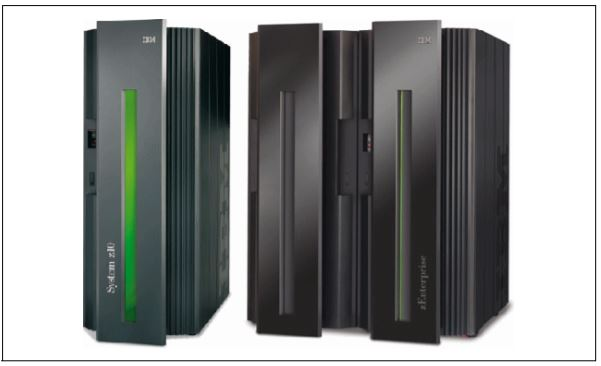
\includegraphics{img/mainframe}
	\caption[Mainframe z13 en LinuxOne Rockhopper]{Een paar mainframes, links de IBM z systems z13 en rechts de LinuxOne Rockhopper}
	\label{fig:mainframe}
\end{figure}



\section{Logische partities en de Parallel Sysplex}
\label{sec:Logische partities en de Parallel Sysplex}

Nu men weet wat een mainframe is, is het belangrijk om te kijken naar de architectuur binnen het systeem zelf. Dit is aan de hand van allerlei gekoppelde logische partities die men als geheel de Parallel Sysplex noemt. Dit is ook de omgeving waarin z/OS Health Checker opereert. Daarom belichten we ook deze componenten in dit hoofdstuk.

\subsection{Logische partitie of LPAR}
\label{subsec:Logische partitie of LPAR}
De IBM mainframe kan verdeeld worden in verscheidene logische systemen. Tussen deze systemen kan men volgende resources verdelen:
\begin{itemize}
	\item Memory
	\item Processors
	\item Input-Output devices.
\end{itemize}
Deze aparte systemen noemt men een logische partitie of LPAR. Al deze LPARs staan onder de controle van een hyperisor. De hypervisor is een software laag voor het beheer van meerdere besturingssystemen. De Verdeling van resources gebeurt door de Processor Resource/Systems Manager(PR/SM). De volledige definitie van een LPAR luidt als volgt: Een subset van de processor hardware dat gedefinieerd is voor het ondersteunen van een besturingssysteem. Meerdere LPARs zijn dus gelijkaardig aan verschillende aparte mainframes. Ze hebben elk hun eigen besturingssysteem. \cite{Ebbers2011}

\begin{figure}[h]
	\centering
	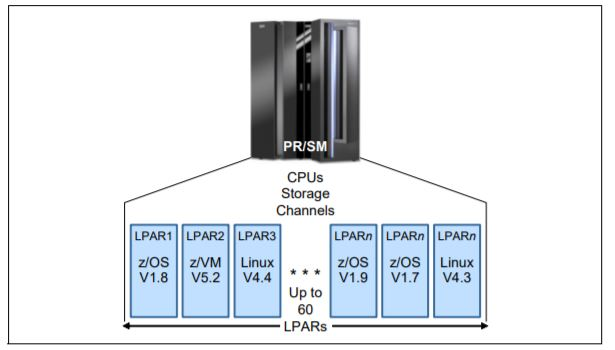
\includegraphics{img/LPAR}
	\caption[Logische Partities]{Visualisatie van logische partities}
	\label{fig:lpar}
\end{figure}


\subsection{Parallel Sysplex}
\label{subsec:Parallel Sysplex}

De Parallel Sysplex is een een techniek van clusteren. Waarmee men meerdere LPARs groepeert.  z/OS Health Checker zal zowel opereren op aparte LPAR als op de gehele Parallel Sysplex door globale checks(meer hierover in \ref{sec:z/OS Health Checker}). Daarvoor gaan we ons ook verdiepen in deze clustering techniek.

Sysplex staat voor SYStems comPLEX dit is een of meerdere LPARs met z/OS, samengevoegd als 1 unit die gespecialiseerde hardware en software gebruikt. Het gebruikt unieke messaging services en kan bestandsstructuren delen in de couple facilty(CF) datasets. Een sysplex is een instantie van een computer systeem dat draait op 1 of meerdere fysieke partities waarvan elke een andere release kan draaien van het z/OS besturingssysteem. Een sysplex is wel geïsoleerd tot 1 fysieke mainframe. De Parallel Sysplex anderzijnds laat meerdere mainframes zich voordoen als 1 systeem. \cite{Ebbers2011} 

Een Parallel Sysplex is een symmetrische sysplex die gebruik maakt van het delen van data met meerdere systemen. Dit is dus de clustering van meerder mainframes. We bespreken ook enkele protocollen die de Parallel Sysplex gebruikt. 

\subsubsection{Server Time Protocol}
\label{subsubsec:Server Time Protocol}

Een belangrijk aspect van de Parallel Sysplex is het synchroniseren van de Time Of Day(TOD) klokken van de meerdere servers. Dit zorgt er bijvoorbeeld voor dat wanneer meerdere servers data aanpassen in de database en er een uitval is. Dat men aan de hand van alle juiste timestamps van de updates van de data de databank kan reconstrueren. Dit gebeurt vandaag met het Server Time Protocol(STP). \cite{Ebbers2011}

\subsubsection{Coupling Facilty}
\label{subsubsec:Coupling Facility}

Sommige z/OS applicaites op verschillende LPARs hebben vaak toegang nodig to dezelfde informatie. Hiervoor betrouwt een Parallel Sysplex op een of meerder Coupling Facilities(CF). Een CF maakt het mogelijk om aan data sharing te doen met meerdere systemen. Een CF is ook een LPAR maar een speciale die andere LPARs toelaat data te delen.

\begin{figure}[h]
	\centering
	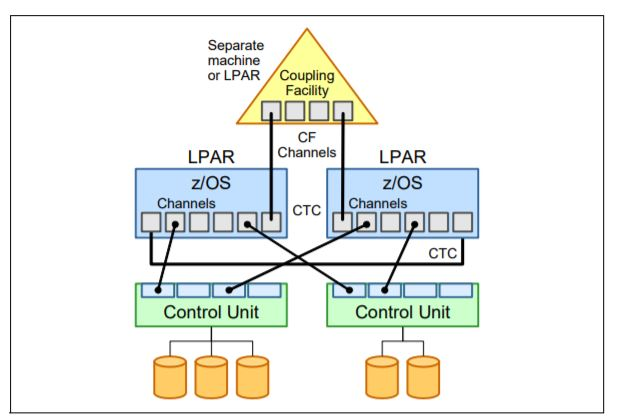
\includegraphics{img/ParallelSysplex}
	\caption[Visualisatie van een Parallel Sysplex]{Visualisatie van een parallel sysplex met 2 LPARs en 1 Coupling Facility. Control Units controleren de logica voor bepaalde I/O-apparaten zoals printers of opslagfaciliteiten in dit geval zijn ze verbonden aan disk drives.}
	\label{fig:parallelsysplex}
\end{figure}


\section{z/OS}
\label{subsec:z/OS}

\section{z/OS Health Checker}
\label{sec:z/OS Health Checker}



